%%%%%%%%%%%%%%%%%%%%%%%%%%%%%%%%%%%%
%%%
%%% Set these variables appropriately
%%%
\newcommand{\AUTHORS}{Torin Rudeen, Samuel Gichohi, and Jonathan Frankle}
\newcommand{\TITLE}{A Framework for Distributed Computer Vision}
\newcommand{\KEYWORDS}{}
\newcommand{\CONFERENCE}{}
\newcommand{\PAGENUMBERS}{yes}       % "yes" or "no"
\newcommand{\TOAPPEAR}{no}
%%%
%%%
%%%%%%%%%%%%%%%%%%%%%%%%%%%%%%%%%%%%

%%%% Setup the document/page
\documentclass[pdftex,twoside,twocolumn,10pt,letterpaper]{article}
\usepackage{ifthen}

\ifthenelse{\equal{\PAGENUMBERS}{yes}}{%
\usepackage[nohead,
            left=1in,right=1in,top=1in,
            footskip=0.5in,bottom=0.75in     % Room for page numbers
            ]{geometry}
}{%
\usepackage[noheadfoot,columnsep=0.2in,
            margin=1in,centering,truedimen]{geometry}
}

\usepackage{fancyhdr}
\usepackage[numbers,sort]{natbib}
\usepackage{xspace}
\usepackage{booktabs}
\usepackage{subfigure}
\usepackage[T1]{fontenc}
\usepackage{textcomp}
\usepackage{mathptmx}   % Times + Times-like math symbols
\usepackage{courier}
\usepackage{enumitem}
\setlist{nolistsep}
\usepackage[scaled=0.92]{helvet}

\usepackage{url}
\def\UrlBreaks{\do\/\do-\do_}

\usepackage{color}
\usepackage[pdftex]{graphicx}
\ifthenelse{\isundefined{\wantBW}}{%
  \usepackage[colorlinks]{hyperref}%        % for online version
}{%
  \usepackage[pdfborder={0 0 0}]{hyperref}% % for paper (B&W) version
}
\newcommand{\URL}[1]{\url{#1}}

%%%%% Setup for PDF
\hypersetup{%
pdfauthor = {\AUTHORS},
pdftitle = {\TITLE},
pdfsubject = {\CONFERENCE},
pdfkeywords = {\KEYWORDS},
bookmarksopen = {true}
}

%\setlength{\parindent}{0pt}
%\setlength{\parskip}{0pt}
\renewcommand{\headrulewidth}{0pt}
\newcommand{\Paragraph}[1]{\vspace{-2ex}\paragraph{#1.}}
\setlength{\topmargin}{-.15in}

\ifthenelse{\equal{\PAGENUMBERS}{yes}}{%
  \pagestyle{plain}
}{%
  \pagestyle{empty}
}

\makeatletter\long\def\@makecaption#1#2{
   \vskip 10pt
   \setbox\@tempboxa\hbox{\textsf{#1: #2}}
   \ifdim \wd\@tempboxa >\hsize % IF longer than one line:
       \textsf{#1: #2}\par      % THEN set as ordinary paragraph.
     \else                      % ELSE  center.
       \hbox to\hsize{\hfil\box\@tempboxa\hfil}
   \fi}
\makeatother

\clubpenalty=10000  % Don't allow orphans
\widowpenalty=10000 % Don't allow widows

\title{\textbf{\TITLE}}
\author{\AUTHORS}
\date{}

% Compact itemize and enumerate.  Note that they use the same counters and
% symbols as the usual itemize and enumerate environments.
\def\compactify{\itemsep=0pt \topsep=0pt \partopsep=0pt \parsep=0pt}
\let\latexusecounter=\usecounter
\newenvironment{CompactItemize}
  {\def\usecounter{\compactify\latexusecounter}
   \begin{itemize}}
  {\end{itemize}\let\usecounter=\latexusecounter}
\newenvironment{CompactEnumerate}
  {\def\usecounter{\compactify\latexusecounter}
   \begin{enumerate}}
  {\end{enumerate}\let\usecounter=\latexusecounter}

\newcommand{\comment}[1]{\textcolor{red}{#1}}
\newcommand{\ignore}[1]{}

\newcommand{\xc}[1]{\mbox{\textit{#1}}}
\newcommand{\la}{\leftarrow}
\newcommand{\ra}{\rightarrow}
\newcommand{\somespace}{\hspace{0.1cm}}

\def\discretionaryslash{\discretionary{/}{}{/}}
\def\discretionarydot{\discretionary{.}{}{.}}
\def\discretionarycolon{\discretionary{:}{}{:}}
{\catcode`\/\active
\catcode`\.\active
\catcode`\:\active
\gdef\URLprepare{\catcode`\/\active\let/\discretionaryslash
                 \catcode`\.\active\let.\discretionarydot
                 \catcode`\:\active\let:\discretionarycolon
        \def~{\char`\~}}}%
\def\URL{\bgroup\URLprepare\realURL}%
\def\realURL#1{\tt #1\egroup}%

\newcommand{\eg}{{\em e.g.}, }
\newcommand{\ie}{{\em i.e.}, }
\newcommand{\etal}{{\em et al.\ }}

\def\check{\stackrel{{\scriptscriptstyle ?}}{=}}

\begin{document}
\maketitle

% -*-LaTeX-*-
% $Id: abstract.tex 70 2007-01-30 21:59:16Z nicolosi $

\begin{abstract}
Recent advances in low-cost, high-performance processors and
computer vision have set the stage for a variety of innovative devices
and applications.  Inspired by the concept of a new generation of
security cameras, we present a C++ and Python framework for
conveniently managing distributed systems of computers equipped
with cameras.  Users define transformations on streams of video
frames, with the framework handling the requisite networking
components and data aggregation.  Initially, the framework eagerly
applied transformations to all frames, the results of which it pushed
to a recipient server.  A subsequent extension allows clients to use an
HTTP-based interface to pull data from cameras, triggering lazy
transformation application.
\end{abstract}

   
\section{Introduction}
\label{sec:intro}

Over the past few years, we have been the beneficiaries of
two quietly game-changing technological revolutions: the coming
of age of low-power processors and computer vision.  While
much of the world's attention has been devoted to Instagram
and Snapchat, cell phone processors silently crossed the 1Ghz
and dual-core marks; recently, Samsung announced an eight core
processor intended for use in high-end smartphones~\cite{exynos}.
Where, as recently as 2007, the flagship cell phone coming to market
was a flip-phone~\cite{razr}, today's smartphones now rival tablets - 
or even laptops - in their computational capabilities.  For use in such
platforms, these processors are also cheap and exceedingly power-efficient.

Although they have mainly seen use in smartphones, these CPUs have
found their way into a variety of other environments where cost and
energy-efficiency are requirements.  One device, the Raspberry Pi,
leverages these developments in inexpensive hardware to supply a
general-purpose computer at a price well under \$50 and in a package
little larger than a pack of playing cards~\cite{pi:faqs}. Online guides exist
for turning the device into everything from a media player appliance
or a sophisticated sensor to a fully-functional desktop machine~\cite{pi:ideas}.
We envision a new application for these inexpensive yet powerful computers
based on recent developments in computer vision.

Computer vision, the process of algorithmically interpreting images to
extract knowledge about their content, has, in the past decade, grown
from a pure research endeavor into a useful toolkit for developers.
OpenCV is an open-source computer vision library compatible with all major
desktop operating systems and with implementations for C++, Python,
Java, and other languages.  It provides a convenient interface for
programmers with limited domain-specific expertise to develop applications
with significant vision components~\cite{cv:about}. Beyond simple ease-of-use,
the library's vision algorithms are highly optimized to be performance-friendly.
OpenCV's success is a major milestone for computer vision research, marking
its ascendance into the ranks of core computer science knowledge.

Connecting the dots, computer vision is getting ever less demanding as
cheap processors are becoming increasingly capable.  We see a world
of possibilities in the intersection of these two trend lines, pairing cameras
with Raspberry Pi-class devices to unlock the imaginations of developers
and enable a variety of new applications.  In this paper, we describe the
design and implementation of a framework for distributed systems of these
computer-equipped cameras that:

\begin{enumerate}
    \setlength{\itemsep}{5pt}
    \item Uses inexpensive, commodity computer and network hardware.
    \item Allows developers to write simple vision algorithms that are applied across the system.
    \item Executes these algorithms efficiently while automatically managing the limited resources of these inexpensive computers.
    \item Makes the results of these algorithms accessible in a convenient, high-level manner.
\end{enumerate}

We first describe the original inspiration for this framework, smart security cameras
(Section 2), and an initial eager, "push" architecture that supports this application (Section 3).
We then explain an extension of this original framework into a lazy, "pull" architecture with an
HTTP-based interface and better resource utilization (Section 4).
\section{Motivation}
If we were to consider the essential requirements of an
effective security camera, what would our list look like?
We know that they would have to take pictures and
rapidly transmit them to a central server.  We would desire
this process to be resilient to network and camera failure,
storing frames persistently and transmitting them as soon
as the network comes back up.  In the event that the network
is congested, they should send the most "important" frames
first, ensuring that critical information reaches the server as
soon as possible.  Physically, they should be easy to install and remove,
providing flexibility and mobility.  Above all, they should be cheap.

It may seem surprising to note that commercially available
security camera solutions satisfy only one of these requirements:
they take pictures.  These systems rely on dedicated, proprietary
physical links or wireless networks, limiting flexibility and increasing
costs.  They demand favorable environments in which congestion
is non-existent, connection speeds are always sufficient, and all processing
can be done instantaneously at the server.  To guarantee these
conditions, manufacturers limit the number of "channels," and therefore
simultaneous cameras, their systems will support.  Even with all of these 
limitations, security camera systems are still quite expensive, with a
\$100/camera price at the lower end of the market.  Most camera
packages tout features like camera quality and access over the internet and
via smartphone apps.

All told, this perfect confluence of ideal circumstances does not hold in
many situations.  Conditions where cameras must be quick to install or even mobile, the 
connection medium is shared, and the link itself is unreliable abound in a variety 
of contemporary settings where video monitoring is essential.  From outdoor 
events to war zones, many environments contain one or more of these adverse 
components that traditional security systems could not overcome.  Furthermore, 
an ideal environment quickly becomes adverse when its owner loses physical 
control, as evidenced in the recent attack at a shopping mall in Nairobi among 
numerous other incidents in the past few years.

We believe that, using an array of Raspberry Pi devices with camera attachments
(\$70 on Amazon at the time of writing), we can develop - at lower cost - a more
robust, flexible, and intelligent security system that is able to continue to meet
these more stringent requirements.  A camera would run feature-detection on each frame it captures,
comparing it to its predecessor and scoring it based on the difference.  Frames with higher
scores would be sent first, with all others cached on persistent memory
until there is enough network bandwidth to send them.  The system could communicate
over a standard 802.11 wireless network, rendering cameras mobile within wireless range
while imposing no strict limit on the number of channels available.  Our framework was
designed with this example in mind, although it has been generalized to support arbitrary
distributed computer vision.

\label{sec:motivation}
\section{Push Architecture}

\paragraph{Dataflow.}

The flow of data through this framework is quite similar to that of MapReduce~\cite{mapreduce}.
Each camera produces a stream of frames, each of which is eagerly passed
through a \emph{transformer} in serial order.  This transformer corresponds to
the mapper in MapReduce: it applies an operation to each frame, producing
zero or more \emph{sendables}.  Unlike MapReduce, however, the transformer may be
stateful, storing information about previously seen frames to inform future decisions.
Transformer state is not saved across executions of the camera program.

Sendables are user-defined objects whose exact
characteristics are unknown to the framework.  They encapsulate the data extracted
from each frame the transformer sees.  Each sendable
must be serializable and deserializable and contain a score property.  The
framework repeatedly serializes the sendable with the highest score and sends
it to the recipient server, hence the term "push."  Use of the score property enables reordering of sendables
by relative importance; to send them in temporal order, a user need only set the
score to the sendable's creation timestamp.

Example transformers include a stateful object that uses feature-detection to assign scores
based on the differences between frames as described in Section 2 and
one that extracts all faces from an image.  Both of these transformers use sendables
that merely store a single image.  We could also imagine a transformer that performs facial recognition
of a specified person or group of people, producing a sendable containing a person's name -
and thereby alerting a remote server - whenever someone is identified in a frame.

\paragraph{Programmer Interface.}

Writing an application that uses the framework is a very straightforward
task for a developer with basic knowledge of any computer vision library such as, OpenCV.  All of the
networking and distributed-systems aspects of the program are automatically
taken care of by the framework.  A programmer must simply extend two
abstract C++ classes: Transformer and Sendable, and compile them into
\emph{Camera} and \emph{Recipient} binaries.

Recipient, executed at the
central server, connects to a camera by TCP port and IP address, listening
for sendables.  Camera, run on each camera node, waits for a Recipient to
connect to a TCP port specified as a command-line argument, after which it
supplies sendables as quickly as possible using the frames it captures.  The
Recipient serializes and stores these sendables to disk.  Each camera uniquely
identifies itself with an integer id that is also dictated by a user on the command-line.
Since cameras listen on TCP sockets, it is possible to retrieve frames from a camera
anywhere on the internet, although it might be difficult to do so over an internet
connection at a reasonable frame rate.  This question is addressed further in the
section about the pull architecture.

When a recipient closes a connection, the camera to which it was formerly connected
waits for another recipient to connect.  Correspondingly, a recipient continuously
attempts to reconnect to the specified camera in the event that its socket closes.


\paragraph{Design}

The design of the push architecture resembles the paradigm described in
SEDA~\cite{seda}, with a multi-stage pipeline of thread pools connected
by bounded queues. The threads in each stage wait on condition variables
when their input queues are empty or their output queues are full.  This
choice avoids wasting CPU cycles spinning on locks while reducing the severity
of lock contention between threads.  Although the effects of condition variables
are decribed in more detail in the evaluation section, this seemingly minor
decision paid tremendous performance dividends in settings where CPU
performance was limited.

In the first stage of the pipeline, frames originate at the camera, from which they
are retrieved and passed through a transformer object in serial order.  A
new frame is not obtained until after the transformer has finished with the
previous one, meaning that the programmer is free to make decisions about
the tradeoff between the camera's frame-rate and the transformer's
computational demands.

Each sendable that a transformer produces receives
a Lamport timestamp that uniquely identifies it.  To ensure that timestamps are
never repeated, even across crashes, the camera uses a range of timestamps in memory while
persistently storing the end of that range in a manner similar to Percolator's
timestamp oracle~\cite{percolator}.  The serialized content of each sendable
is passed through a FIFO queue to a thread pool that stores them persistently,
while its metadata is added to a priority queue ordered by score.  By storing only
metadata in memory, the framework keeps its memory footprint as small as possible to ensure it can
endure a significant backlog of sendables even on devices with limited RAM
like Raspberry Pis.  Temporarily storing sendables in progress to disk also allows the
camera's backlog to persist across crashes.

Another thread pool retrieves sendable metadata from the priority queue, pulling
those with highest scores first, and loads their serialized contents from disk into
memory, adding this information to a bounded "sending queue" in preparation for transmission
over the network.  If the sending queue is full, the threads wait until there is again
room to retrieve more sendables.  As an optimization to avoid unnecessary disk
reading and writing, sendables may take a "fast path" and be moved from the transformer
directly into the sending queue if the priority queue is empty and the sending queue is not full.
This queued approach minimizes the memory presence necessary to guarantee that
the network never has to wait on disk accesses;
multiple threads fetching sendables simultaneously mask this delay.  Since Raspberry Pis
rely on SD cards as their primary hard drives, the time necessary to load sendables from
disk could be significant.

A single thread reads from the sending queue and transmits serialized sendables and their
Lamport timestamps over the network.  A final thread listens for the recipient to
echo the timestamps, which serves as an acknowledgement that the data has
been received and persistently stored.  Once acknowledged, sendables are deleted
from the camera's disk to free up space.  Users of the framework may optionally
place a limit on the number of sendables that are simultaneously in-flight; if this
cap has been met, the sending thread waits for additional acknowledgements
before transmitting further sendables.

\paragraph{Fault Tolerance}

The push architecture is robust to transient failures of both the network and the
camera itself.  All sendables are saved persistently upon creation, meaning that
the priority queue of metadata can be reconstructed from disk after a crash.
Sendable creation continues regardless of the state of the network; if the network
is down, the camera can catch up by transmitting old sendables when it is working again.
Since Lamport timestamps are doled out in ranges, with the top of the range stored
on disk, timestamps will remain unique across crashes, even if many numbers may be
skipped in the process.  Sendables are not deleted from disk until they are individually
acknowledged by a recipient, providing for retransmission of sendables lost due to
network errors or crashes while sending is in progress.  Although these safeguards
impose additional overhead, making such guarantees is essential for applications like
the security camera described in Section 2.

\paragraph{Evaluation}

We tested the framework's ability to send frames over the over the network
using two different transformations: one that makes no modifications
(Identity) and one the reorders frames using feature detection on up to
100 features (Feature Delta).  The benchmarks were conducted over a
virtual network supported by VirtualBox with a tested network speed of about 1.5Gbps.
We used traffic shaping to simulate a network at capacities between 1Mbps and 12Mbps in order to
determine the point at which the framework's bottleneck switches from being the
network bandwidth to the camera's CPU or maximum frame rate.  The camera machine had 4GB of RAM
and ran an Intel Core i5-2410M, which has two cores (four logical cores with HyperThreading)
and a maximum sustained clock speed of 2.3GHz.  The recipient
ran on a virtual machine on the same computer.  The camera's maximum possible
frame rate through OpenCV was measured at slightly above 15 frames per second.

\begin{figure}[h]
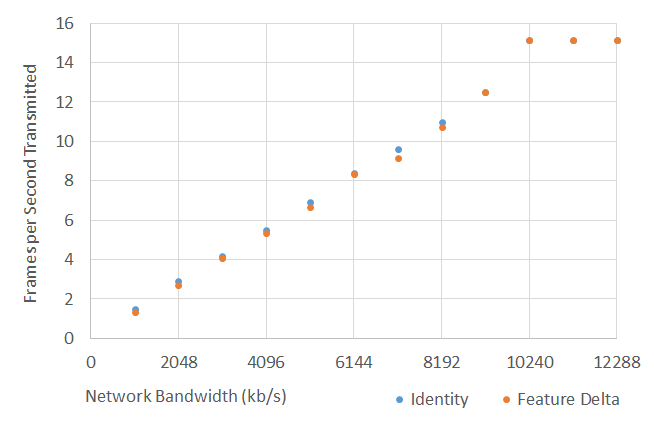
\includegraphics[width=\columnwidth]{figure3.png}
\caption{Framework tests with CPU at 2300MHz.}
\end{figure}

On the first run, the CPU clock speed was set to its maximum value. As Figure 1
demonstrates, the frame rate was proportional to the network speed at bandwidths
below 10Mbps, indicating that the network was the bottleneck.  At higher speeds,
the graph flattens as the camera reached its maximum possible frame rate.
There was no tangible difference in the frame rates between the operations,
showcasing the performance efficiency of the feature detection operation.

\begin{figure}
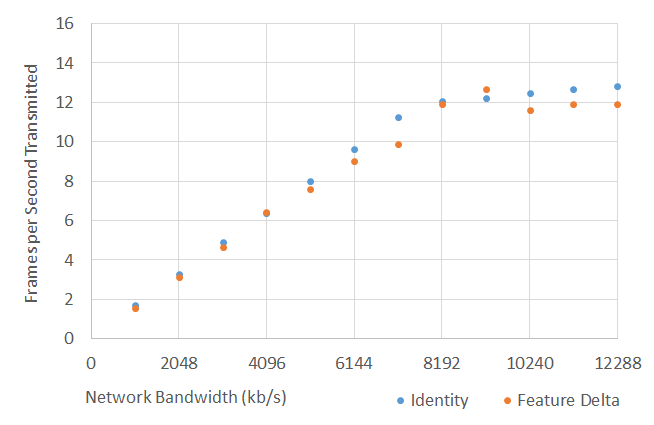
\includegraphics[width=\columnwidth]{figure4.png}
\caption{Framework tests with CPU at 800MHz.}
\end{figure}

With the clock speed throttled to 800MHz, the results were little different.  Up to about
9Mbps, the transmitted frame rate was quite close to that measured at 2300MHz.  At
higher bandwidths, the frame rate again flattened, this time about 2 frames per second
lower than in the first test.  As before, there was only a slight decrease in performance
between the two transformations.  Even in this test, the CPU usage remained well
below 100\%.

Although we have no direct basis for comparison between the Core i5 processor in the
test camera and the Raspberry Pi's ARM CPU, we can safely conclude that this framework
supports vision algorithms that run efficiently on computationally limited hardware, providing
acceptable frame rates even at relatively low network bandwidths.  The framework's transmission rate
is mainly network and camera-sensitive, giving us confidence that
this framework  will easily translate to high-end cell phone processors.

\begin{figure}
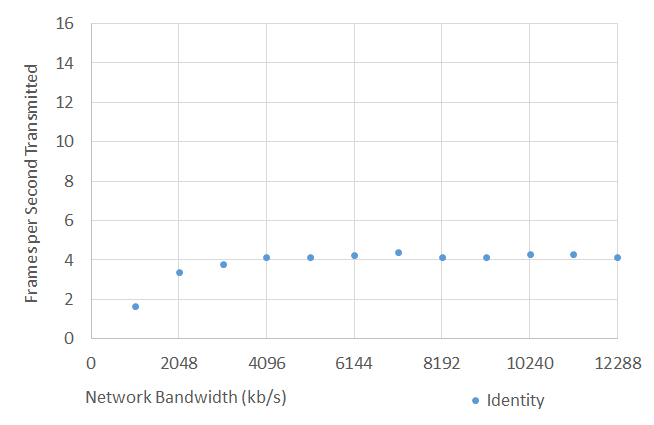
\includegraphics[width=\columnwidth]{figure5.png}
\caption{Identity transformation with CPU at 800MHz and spinning on locks rather than condition variables.}
\end{figure}

Interestingly, the original implementation of the push architecture required each pipeline stage to
spin on locks while waiting for information to enter its queue.  A subsequent iteration, the
one used to produce the data above, replaced this spinning with condition variables, resulting
in a 3x to 5x improvement in frame rates and significantly lower CPU utilization across all tests.
Figure 3 displays the frame rates from the Identity transformation using spinning on locks with
the processor speed set at 800MHz.  As
the graph clearly demonstrates, the simple change in synchronization primitive had a dramatic impact on
the overall performance of the framework.

\section{Pull Architecture}
\label{sec:pull}

\paragraph{Limitations of the Push Architecture.}
The most significant weakness of the push architecture is
that it eagerly applies a transformation to all frames, creating
many sendables that, due to network limitations, may never
actually be transmitted.  This unnecessary computational work is
potentially significant on a device like a Raspberry Pi. The
push architecture also presents a difficult-to-use
interface to a programmer writing a recipient server, which
must efficiently handle a continuous flow of sendables.
These two deficiencies inspired an extension of the original
architecture into one which lazily applies transformations and
presents an HTTP-based interface to recipients, resulting in a
more efficient and usable framework.

\paragraph{Design.}
Although performing all transformations lazily would achieve
optimal efficiency by only doing work that is absolutely necessary,
solely permitting lazy transformations would render global sendable
reordering impossible.  We therefore took a hybrid approach
where a user supplies two sets of transformations.  The first,
eager transformation is applied as in the push architecture.
Rather than doing all of the work, the eager transformation
should be written so as to efficiently do any reordering and
data size reduction that must be applied globally.  These
\emph{intermediate sendables} are inserted into a database, where
they are accessible to a number of more work-intensive, lazy
transformations.  Data recipients can then request the final
results of these transformations over HTTP.  This compromise
between laziness and eagerness maintains the best aspects
of the original model while compensating for its weaknesses.

\paragraph{Programmer Interface}
These changes represent a pure extension to the original framework.
Rather than pushing sendables over the network, the original model
was modified to insert them, along with other metadata, into a SQLite
database.  This database is made accessible to a webserver interface
written in Python.  Users of the framework write Python functions
that encapsulate different queries a recipient might make on a lazy
transformation, such as performing it on the highest-scored sendable
available or sendables created between 2:00pm and 3:00pm.  This
Python section of the framework exports URLS of the format:

\texttt{\\http://[ip]/do/[function]?[arguments]\\}

The \texttt{function} component of the URL refers to the name of
the Python function to be executed.  Recipients supply arguments to the method using
the URL's query string.  Users of the framework are free to either
pass the results of the transformation in response to the original HTTP
message or to respond with a second URL from which the results are accessible.
Since Python has first-class functions, programmers can easily 
combine transformations.

\paragraph{Enhancements}

In addition to optimizing the performance of the framework,
this extension supports several additional enhancements.  Users may 
define multiple transformations that run in parallel on each camera and
examine cameras from any number of recipients.  These transformations
have free reign over the database of sendables, permitting
the framework to transparently support sendable-specific queries that
would previously have been impossible.   The pull architecture provides a
convenient interface at a high level of abstraction for the framework, making
it far easier to use than the push architecture alone.

Finally, the push architecture presents a much more useful interface
for a user wishing to examine the state of a camera over the interent.
To do so with the push architecture would have required a viewer to receive
and store all frames that a camera supplied, which would be highly inconvenient on
a smartphone app.  The pull architecture permits a user to perform queries on
the state of a camera without receiving an overwhelming amount of data or
modifying the state of the camera in any way.

\section{Related Work}
\label{sec:related}

There has been significant previous work on video analysis and keyframe
detection in the computer vision community. For example, Girgensohn and
Boreczky \cite{related1} accomplish this process by applying a clustering
algorithm to the set of frames from a video and selecting a representative
frame from each cluster. Wolf \cite{related2} first divides the video into shots by detecting 
camera cuts and transitions, and then looks for local minimums of object motion
within each shot, presenting these as the keyframes. These approaches are
not a good fit for our problem, as they either only work offline, or are based
on assumptions about how videos are shot that only hold true for media
professionally produced for entertainment. 

There has also been research into applying computer vision to analyze
security footage, but it focuses on semantic analysis of large archives of
video, rather than on determining individual frames that are not important.
For example, Regazzoni’s work \cite{related3} finds abandoned objects in
video footage to help police searching events like, for example, the moment
when a bomb was planted. 

For the Feature Delta transformer, we used an approach based on applying
the SIFT feature detector \cite{related4} to find features within each frame
and then assigning importance to frames where new features arise
or existing features move significantly. This approach is simple and fast,
can use existing implementations of the SIFT algorithm, and is
not based on a particular semantic interpretation of the scene.



\section{Conclusions}
\label{sec:conclusion}

We have designed and implemented a framework for distributed
computer vision that allows programmers to easily write their own
applications using domain-specific expertise.  The framework achieved
and exceeded our original goal of building a smart security camera system,
facilitating the development of that and several other sample algorithms.  The framework
comes in two varieties: one that pushes data to a recipient as rapidly as
possible and one that supplies an HTTP-based interface for interacting with
data the camera has collected.  Our performance tests show that, even
in environments where computational power is quite limited, the framework
still achieves frame rates that are limited only by the speed of the network and
the camera itself.  We are excited by the new class of possible
applications that this framework, combined with powerful, inexpensive
hardware and advances in computer vision, has enabled.

%% Bibliography
%\vspace{-1ex}
%\linespread{1.0}
%\setlength{\bibsep}{1pt}
%\footnotesize
\small
\bibliographystyle{abbrvnat}
\bibliography{local}


\end{document}

